\chapter{How to draw spherical harmonics} \label{app:A}

\section{The spherical harmonics}
For the first time students encounter spherical harmonics, we are most likely
scared away by the complicated expressions and bizarre geometries of the plots.
Complaining,
\begin{quote}
``I can never understand these functions and crazy plots. It's all so complicated!''
\end{quote}

This is, however, always the case when we learn something new. Things usually look
incomprehensible until we understand them and set up a good friendship.

Spherical harmonics are the solutions of the angular equation in (\ref{eq:YEqn}):
\begin{equation} \label{eq:YEqnAppend}
\frac{1}{\sin{\theta}} \frac{\partial}{\partial \theta} \left( \sin{\theta} \frac{\partial Y}{\partial \theta} \right) + \frac{1}{\sin^2{\theta}} \frac{\partial^2 Y}{\partial \phi^2} = -l(l+1) Y
\end{equation}
%
The derivations are nicely discussed in Griffiths' book \cite{QM}. In this short appendix,
we are not going to repeat the derivations, but will emphasize another interesting
perspective: how to draw the spherical harmonics. Not only for impressing your friends,
but more importantly, once we understood how they are plotted,
we will get a direct feeling of spherical harmonics and essentially comprehend their meanings.

The spherical harmonics $Y_{lm}(\theta,\phi)$ (with $l=0,\ 1,\ \ldots$ and $m=-l,\ \ldots,\ l$),
are given by
\begin{equation} \label{eq:sphaAppend}
Y_{lm}(\theta,\phi) = \sqrt{\frac{2l+1}{4\pi}\frac{(l-m)!}{(l+m)!}} P_l^m(\cos{\theta}) e^{im\phi}
\end{equation}
The big square root in front is nothing but a normalization factor, simply a real number.
The exponential term in the end is called the phase, which never contributes when we
consider the modulus square $|Y_{lm}|^2$. Probably the most scaring term is $P_l^m$, the
associated Legendre polynomials. But don't worry, they can be computed very easily. The computation
routine is clearly provided by \emph{Numerical Recipes} \cite{NR}. To give a direct impression,
Table~\ref{table:Ylm} explicitly listed the first few spherical harmonics.

\begin{table}[h!]
\caption{The first few spherical harmonics $Y_{lm}(\theta,\phi)$.}
\label{table:Ylm}
\begin{equation*}
\renewcommand\arraystretch{2.2}
\begin{array}{|>{\displaystyle}r >{\displaystyle}r >{\displaystyle}l >{\displaystyle}l|}
  \hline
  Y_{0,\phantom{\pm}0} = & \sqrt{\frac{1}{4\pi}}      &                                 &  \\[0.4em] \hline
  Y_{1,\phantom{\pm}0} = & \sqrt{\frac{3}{4\pi}}      & \cos{\theta}                    &  \\
  Y_{1,\pm1}           = & \mp\sqrt{\frac{3}{8\pi}}   & \sin{\theta}                    & e^{\pm i\phi} \\[0.4em] \hline
  Y_{2,\phantom{\pm}0} = & \sqrt{\frac{5}{16\pi}}     & (3\cos^2{\theta}-1)             &  \\
  Y_{2,\pm1}           = & \mp\sqrt{\frac{15}{8\pi}}  & \sin{\theta}\cos{\theta}        & e^{\pm i\phi} \\
  Y_{2,\pm2}           = & \sqrt{\frac{15}{32\pi}}    & \sin^2{\theta}                  & e^{\pm 2i\phi} \\[0.4em] \hline
  Y_{3,\phantom{\pm}0} = & \sqrt{\frac{7}{16\pi}}     & (5\cos^3{\theta}-3\cos{\theta}) &  \\
  Y_{3,\pm1}           = & \mp\sqrt{\frac{21}{64\pi}} & \sin{\theta}(5\cos^2{\theta}-1) & e^{\pm i\phi} \\
  Y_{3,\pm2}           = & \sqrt{\frac{105}{32\pi}}   & \sin^2{\theta}\cos{\theta}      & e^{\pm 2i\phi} \\
  Y_{3,\pm3}           = & \mp\sqrt{\frac{35}{64\pi}} & \sin^3{\theta}                  & e^{\pm 3i\phi} \\[0.4em]
  \hline
\end{array}
\end{equation*}
\end{table}

\section{Plotting in spherical coordinates}
Perhaps the most common and easiest way to make a plot is to plot in the Cartesian coordinate system.
Just like how we plotted our radial wave functions $u_{nl}(r)$. We took the $x$-axis representing
our spacial distance $r$ and $y$-axis representing our wave functions $u_{nl}$
\begin{equation} \label{eq:cartesian}
  \begin{cases}
  x \gets r \\
  y \gets u_{nl}
  \end{cases}
\end{equation}

However, for our angular wave functions, namely the spherical harmonics $Y_{lm}(\theta,\phi)$, it is
more natural to plot them in a spherical coordinate system, since it is where they are
defined. Now the mapping is the following,
\begin{equation} \label{eq:spherical}
  \begin{cases}
  r \gets Y_{lm} \\
  \theta \gets \theta \\
  \phi \gets \phi
  \end{cases}
\end{equation}

The important message is that we use the radius to represent the
amplitude of spherical harmonics. The functions listed in
Table~\ref{table:Ylm} are good enough for us to make a couple of
beautiful plots. For simplicity, we would like
to restrict the azimuthal angle $\phi$ to 0,
that is, we plot in the $xz$-plane. So now we have only one variable $\theta$.
To make the plots, we first define our grid in $\theta$
\begin{equation} \label{eq:thetaGrid}
\left\{ \theta_{\text{min}} = 0;\quad \theta_{\text{max}} = 2\pi;\quad \Delta \theta = \frac{\pi}{12}; \right\}
\end{equation}
To get started, let's plot the simplest function $Y_{00}$,

For $\theta=0\,\,\,$, we have $r=\sqrt{\frac{1}{4\pi}}$;\newline
For $\theta=\frac{\pi}{12}$, we have $r=\sqrt{\frac{1}{4\pi}}$;\newline
For $\theta=\frac{2\pi}{12}$, we have $r=\sqrt{\frac{1}{4\pi}}$;\newline
\ldots \newline
For $\theta=2\pi$, we have $r=\sqrt{\frac{1}{4\pi}}$.

If we plot these data points and connect them, we get a circle! (Fig.~\ref{fig:Y00})
\begin{figure}[h!]
\centering
  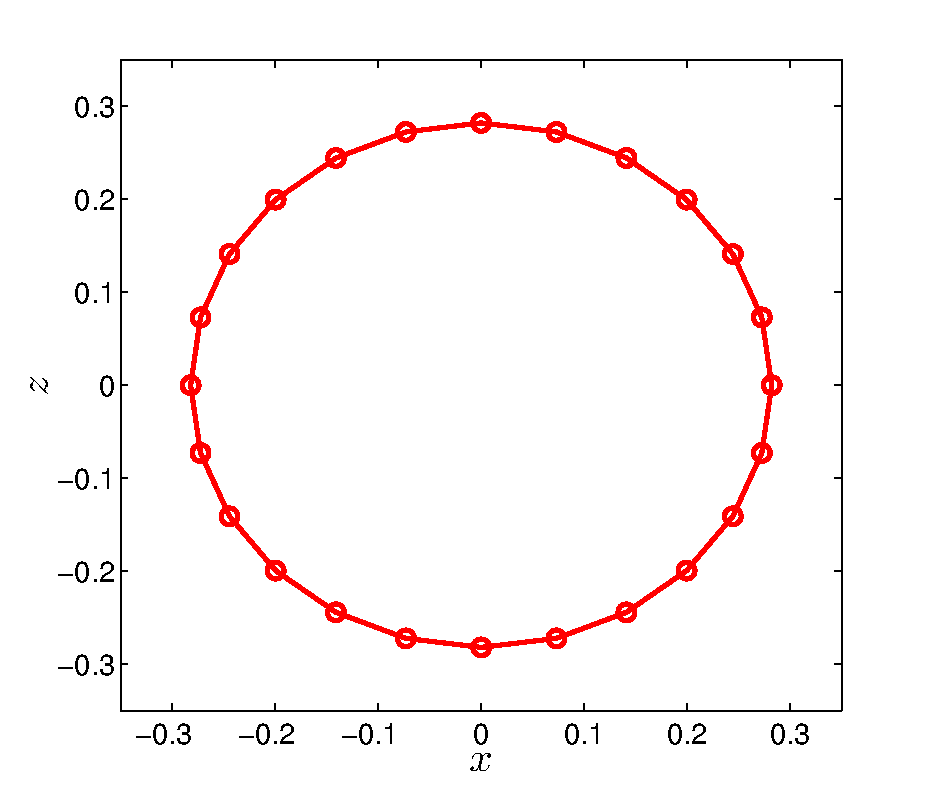
\includegraphics[width=0.36\textwidth,height=0.33\textwidth]{Y00}
  \caption{$Y_{00}(\theta,\phi)$ in the $xz$-plane.}
  \label{fig:Y00}
\end{figure}

$Y_{00}$ was simple enough. Let's try a more exciting one, $Y_{10}$,

For $\theta=0\,\,\,\,\,$, we have $\,\,r \approx 0.4886$;\newline
For $\theta=\frac{\pi}{12}\,\,$, we have $\,\,r \approx 0.4720$;\newline
\ldots \newline
For $\theta=\frac{7\pi}{12}\,\,$, we have $\boxed{r \approx -0.1265}$;\newline
\ldots \newline
For $\theta=\frac{23\pi}{12}$, we have $\,\,r \approx 0.4720$;\newline
For $\theta=2\pi\,\,$, we have $\,\,r \approx 0.4886$.

Wait! how do we plot a negative radius? Hum... we really can only plot the
absolute value. To indicate the different signs, let's use two different colors.
We use red color for positive $Y_{10}$ and blue color for negative $Y_{10}$.
Now we plot the data points and connect them. We get a red-blue colored plot in Fig.~\ref{fig:Y10}
\begin{figure}[h!]
\centering
  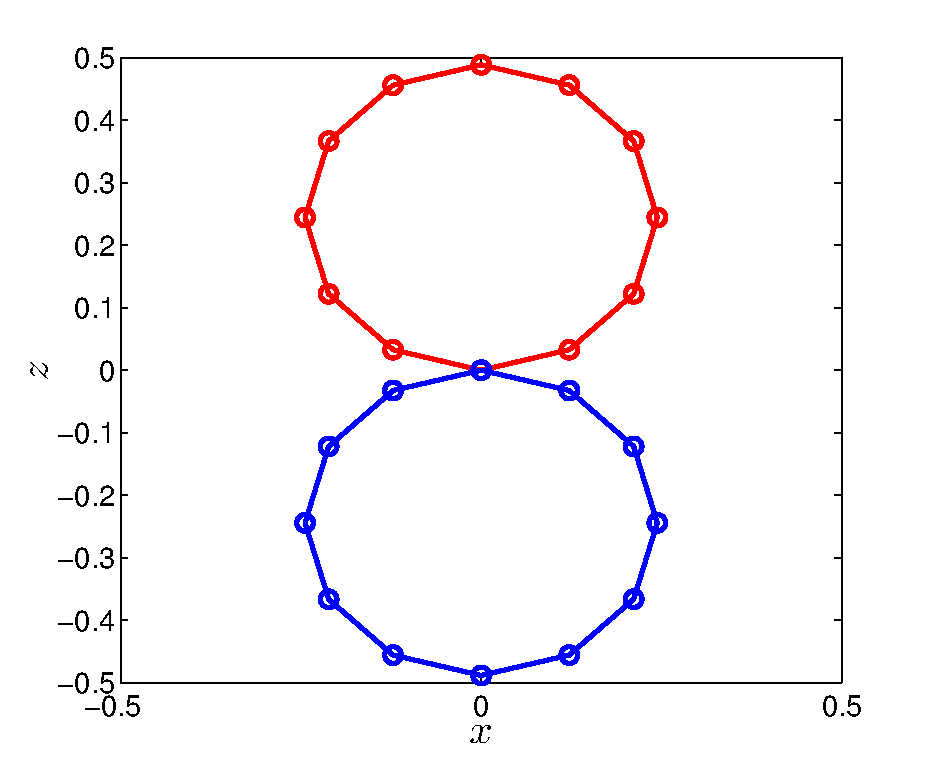
\includegraphics[width=0.36\textwidth,height=0.33\textwidth]{Y10}
  \caption{$Y_{10}(\theta,\phi)$ in the $xz$-plane.}
  \label{fig:Y10}
\end{figure}

The color of the plot doesn't contribute much into the physical meaning.
Never ever misunderstand them as positive or negative charges (or whatever). The physical
meaning is represented by the modulus square of the wave function $|Y_{lm}|^2$,
which is the probability density of finding an electron.
It doesn't really matter which color ($\pm$ sign) it is.

Previously we restricted our azimuthal angle to 0. It wouldn't be too difficult
to extend our discussion for arbitrary $\phi$. When we consider a non-zero $\phi$,
we may have the situation that $Y_{lm}$ is a complex number. But we simply
plot the modulus of the complex number, so it won't be a problem. Nevertheless,
if we want to indicate the phase of the complex number (just like for indicating the $\pm$ sign),
we can do some color mapping to make a fancy plot.
To get an idea how it works, we take the function $Y_{1,-1}$ as an example.
This time, we restrict our inclination angle $\theta$ to $\frac{\pi}{2}$, that is,
we plot in the $xy$-plane. Now we have freedom in $\phi$.
\begin{equation} \label{eq:phiGrid}
\left\{ \phi_{\text{min}} = 0;\quad \phi_{\text{max}} = 2\pi;\quad \Delta \phi = \frac{\pi}{12}; \right\}
\end{equation}
For $\phi=0\,\,\,$, we have $r \approx 0.3455 e^{\phantom{-}0.0000i}$;\newline
For $\phi=\frac{\pi}{12}$, we have $r \approx 0.3455 e^{-0.2618i}$;\newline
For $\phi=\frac{2\pi}{12}$, we have $r \approx 0.3455 e^{-0.5236i}$;\newline
\ldots \newline
For $\phi=2\pi$, we have $r \approx 0.3455 e^{-6.2832i}$.

We plot the modulus of the complex numbers as the radius. And we map the
colors according to the phase angles of the complex numbers,
which is the angle formed by the real and imaginary parts on
the complex plane. The choice of colors is arbitrary, but it is good to have some
continuously interpolated colors to represent the continuous phase angles. (Fig.~\ref{fig:Yphi})
\vspace{-0.5em}
\begin{figure}[h!]
\centering
  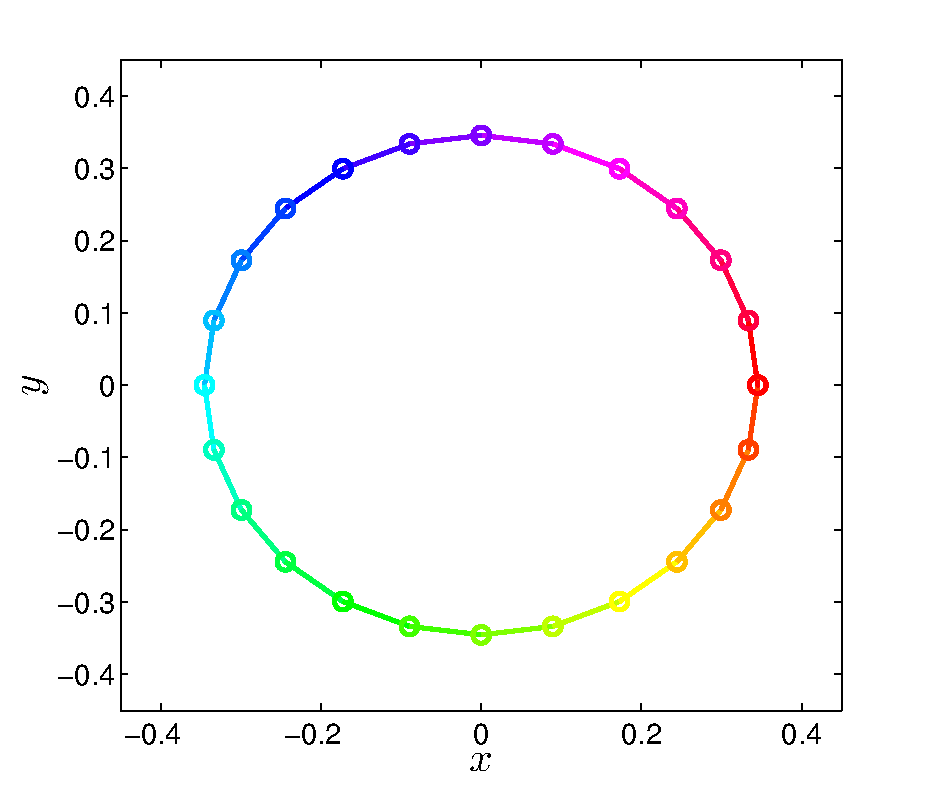
\includegraphics[width=0.36\textwidth,height=0.33\textwidth]{Yphi}
  \caption{$Y_{1,-1}(\theta,\phi)$ in the $xy$-plane.}
  \label{fig:Yphi}
\end{figure}

We have basically introduced all the essential ideas for plotting spherical
harmonics. All that remains is to implement (or use) a 3D visualization program
to visualize the $(r,\theta,\phi)$ data. Writing a 3D visualization program
involves some computer graphics knowledge, such as the coordinate transformations
and shading programs. I have implemented a program using the WebGL technology,
which can be run directly in a modern browser. I summarize some nice plots generated
by WebGL in Table~\ref{table:pureYlm}, which are the functions listed in Table~\ref{table:Ylm}.

\section{Linear combinations of spherical harmonics}
The spherical harmonics $Y_{lm}$ (called pure harmonics)
are solutions from Eqn.~(\ref{eq:YEqnAppend}).
Consequently, their linear combinations (with the same $l$) are also valid solutions.
Actually, you can take any crazy combinations to make some crazy plots.
But there are a handful of pre-defined linear combinations, which are
typically useful for chemists. Those pre-defined
combinations are called real harmonics. Because those
combinations (by combining $\pm m$)
eliminate the imaginary parts and result in
functions which are in the real range. The first few real harmonics
are listed in Table~\ref{table:realHarm}. The corresponding plots
are also given in Table~\ref{table:realYlm}. You will see only two
colors, because there are only positive and negative real numbers!

\begin{table}[h!]
\caption{The first few real harmonics.}
\label{table:realHarm}
\vspace{1em}
\hspace{4em}
\begin{minipage}{0.4\textwidth}
\begin{equation*}
\renewcommand\arraystretch{2.2}
\begin{array}{|>{\displaystyle}l >{\displaystyle}c >{\displaystyle}l|}
  \hline
  s               & = & Y_{0,0}                       \\[0.4em] \hline
  p_z             & = & Y_{1,0}                       \\
  p_x             & = & \sqrt{\frac{1}{2}}\phantom{i}(Y_{1,-1}-Y_{1,1})  \\
  p_y             & = & \sqrt{\frac{1}{2}}i(Y_{1,-1}+Y_{1,1}) \\[0.4em] \hline
  d_{3z^2-1}      & = & Y_{2,0}                       \\
  d_{xz}          & = & \sqrt{\frac{1}{2}}\phantom{i}(Y_{2,-1}-Y_{2,1})  \\
  d_{yz}          & = & \sqrt{\frac{1}{2}}i(Y_{2,-1}+Y_{2,1}) \\
  d_{x^2-y^2}     & = & \sqrt{\frac{1}{2}}\phantom{i}(Y_{2,-2}+Y_{2,2})  \\
  d_{xy}          & = & \sqrt{\frac{1}{2}}i(Y_{2,-2}-Y_{2,2}) \\[0.4em]
  \hline
\end{array}
\end{equation*}
\end{minipage}
\begin{minipage}{0.4\textwidth}
\begin{equation*}
\renewcommand\arraystretch{2.2}
\begin{array}{|>{\displaystyle}l >{\displaystyle}c >{\displaystyle}l|}
  \hline
  f_{z(5z^2-3)}   & = & Y_{3,0}                       \\
  f_{x(5z^2-1)}   & = & \sqrt{\frac{1}{2}}\phantom{i}(Y_{3,-1}-Y_{3,1})  \\
  f_{y(5z^2-1)}   & = & \sqrt{\frac{1}{2}}i(Y_{3,-1}+Y_{3,1}) \\
  f_{z(x^2-y^2)}  & = & \sqrt{\frac{1}{2}}\phantom{i}(Y_{3,-2}+Y_{3,2})  \\
  f_{xyz}         & = & \sqrt{\frac{1}{2}}i(Y_{3,-2}-Y_{3,2}) \\
  f_{x(x^2-3y^2)} & = & \sqrt{\frac{1}{2}}\phantom{i}(Y_{3,-3}-Y_{3,3})  \\
  f_{y(3x^2-y^2)} & = & \sqrt{\frac{1}{2}}i(Y_{3,-3}+Y_{3,3}) \\[0.4em]
  \hline
\end{array}
\end{equation*}
\end{minipage}
\end{table}

\clearpage
\begin{table}
\begin{center}
\small
\rotatebox{-90}{
\begin{minipage}{\textheight}
\caption{The first few pure spherical harmonics.}
\label{table:pureYlm}
\makebox[1.1\textheight]{
\begin{tabular}{c c c c c c c}
& & & 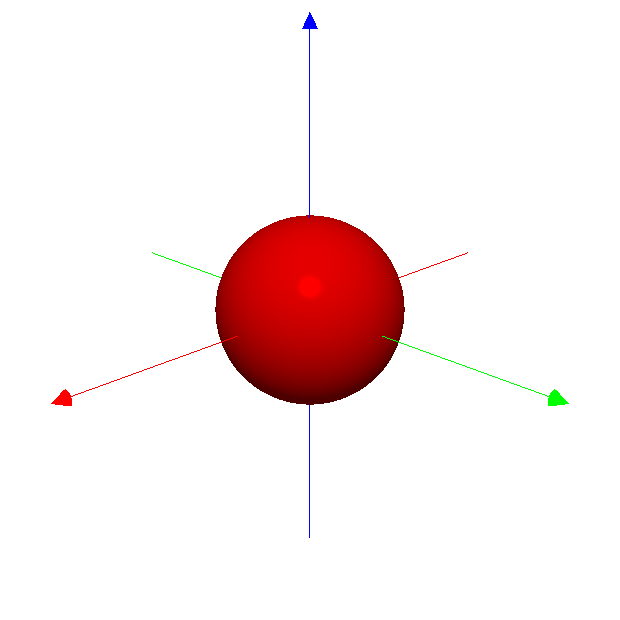
\includegraphics[width=0.14\textwidth,trim={0 3cm 0 -2cm},clip]{00} & & & \\
& & & $l=0,\;m=0$ & & & \\
& & 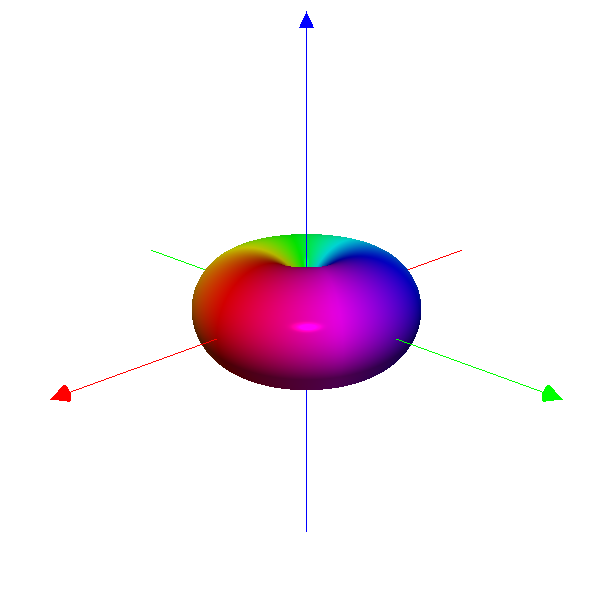
\includegraphics[width=0.14\textwidth,trim={0 3cm 0 -2cm},clip]{1m1} & 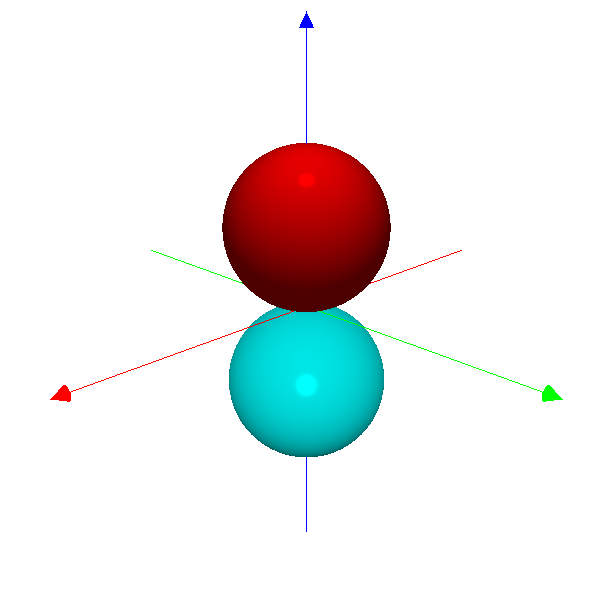
\includegraphics[width=0.14\textwidth,trim={0 3cm 0 -2cm},clip]{10} & 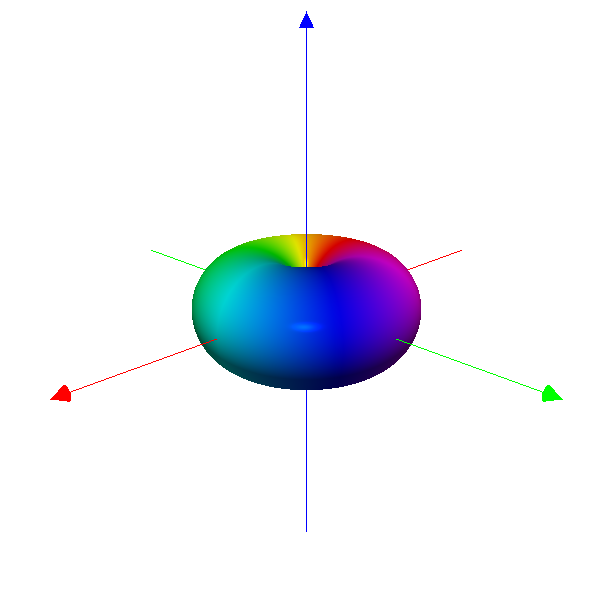
\includegraphics[width=0.14\textwidth,trim={0 3cm 0 -2cm},clip]{1p1} & & \\
& & $l=1,\;m=-1$ & $l=1,\;m=0$ & $l=1,\;m=1$ & & \\
& 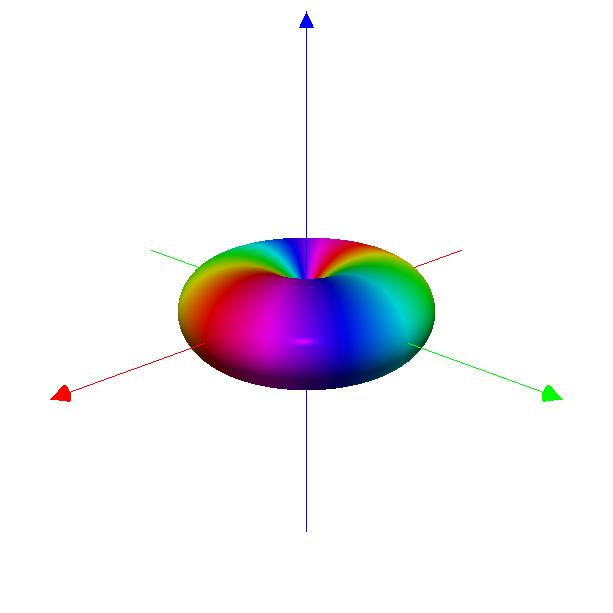
\includegraphics[width=0.14\textwidth,trim={0 3cm 0 -2cm},clip]{2m2} & 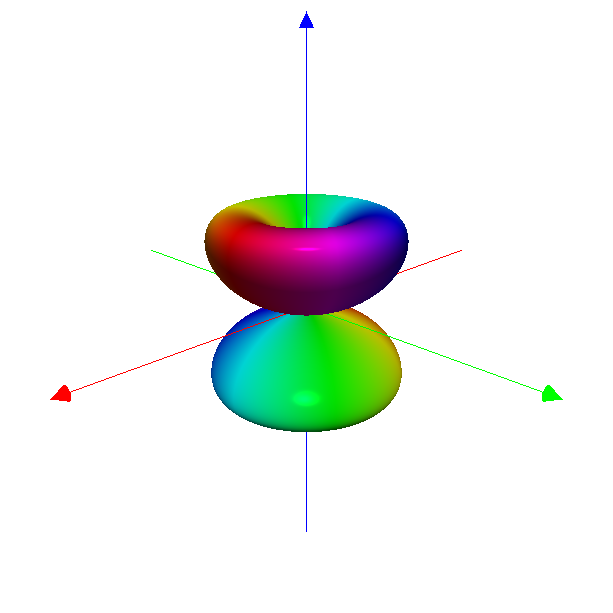
\includegraphics[width=0.14\textwidth,trim={0 3cm 0 -2cm},clip]{2m1} & 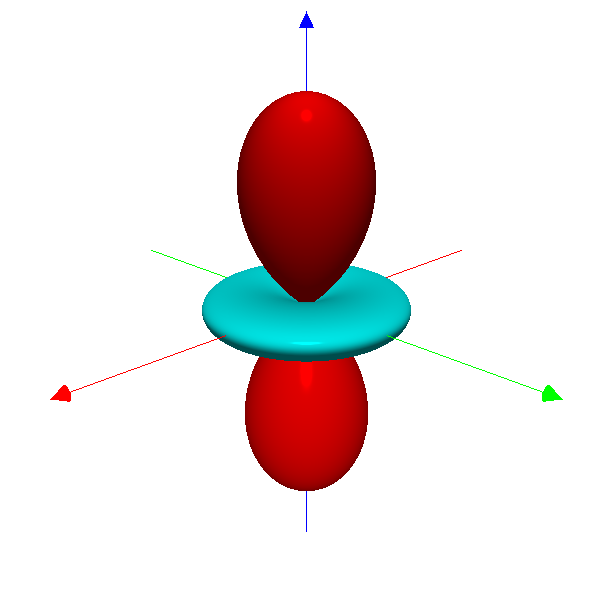
\includegraphics[width=0.14\textwidth,trim={0 3cm 0 -2cm},clip]{20} & 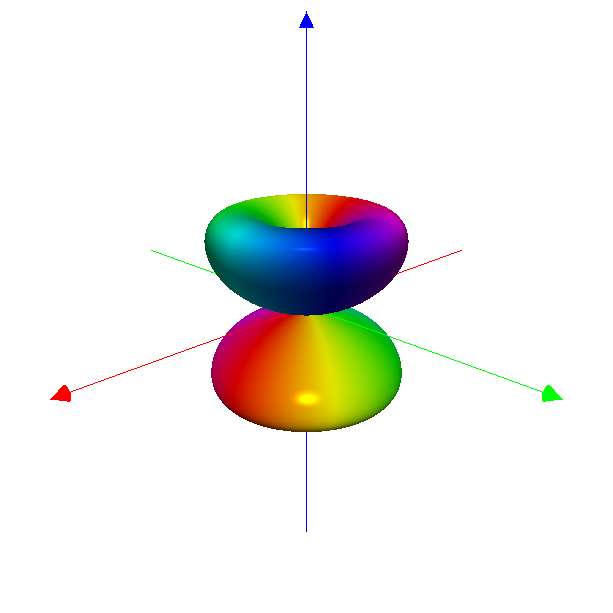
\includegraphics[width=0.14\textwidth,trim={0 3cm 0 -2cm},clip]{2p1} & 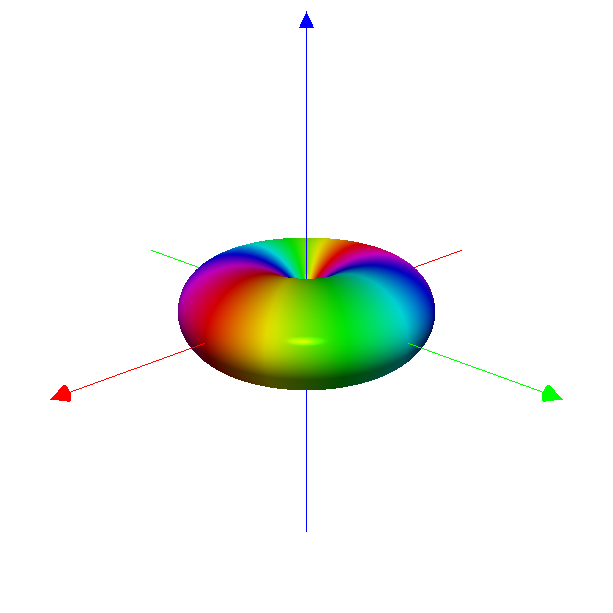
\includegraphics[width=0.14\textwidth,trim={0 3cm 0 -2cm},clip]{2p2} & \\
& $l=2,\;m=-2$ & $l=2,\;m=-1$ & $l=2,\;m=0$ & $l=2,\;m=1$ & $l=2,\;m=2$ & \\
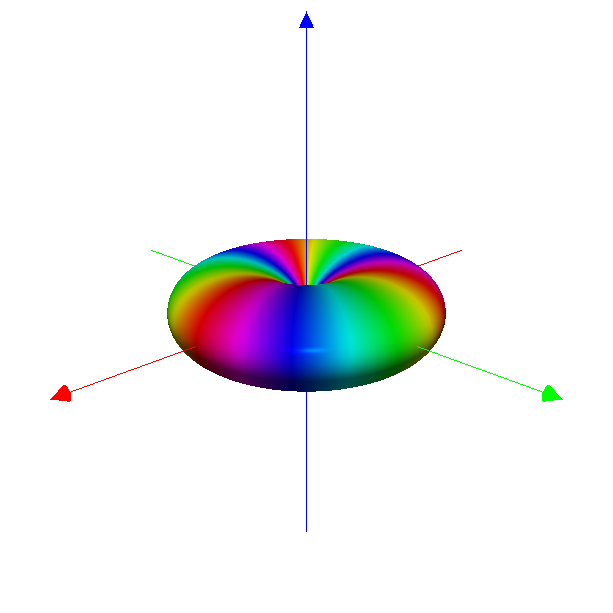
\includegraphics[width=0.14\textwidth,trim={0 3cm 0 -2cm},clip]{3m3} & 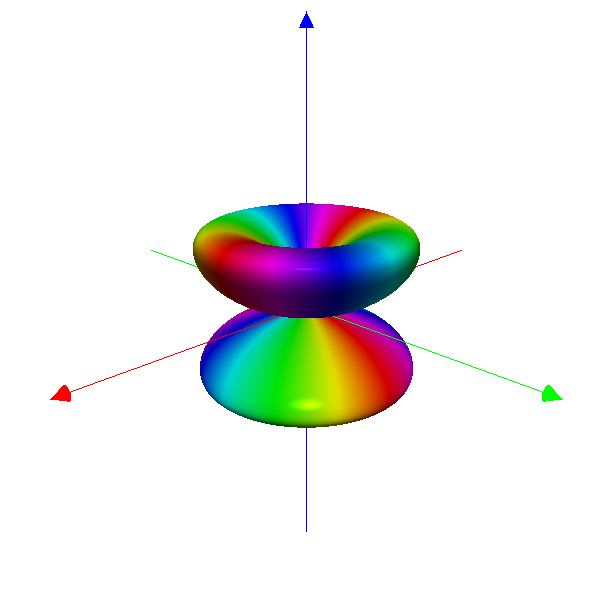
\includegraphics[width=0.14\textwidth,trim={0 3cm 0 -2cm},clip]{3m2} & 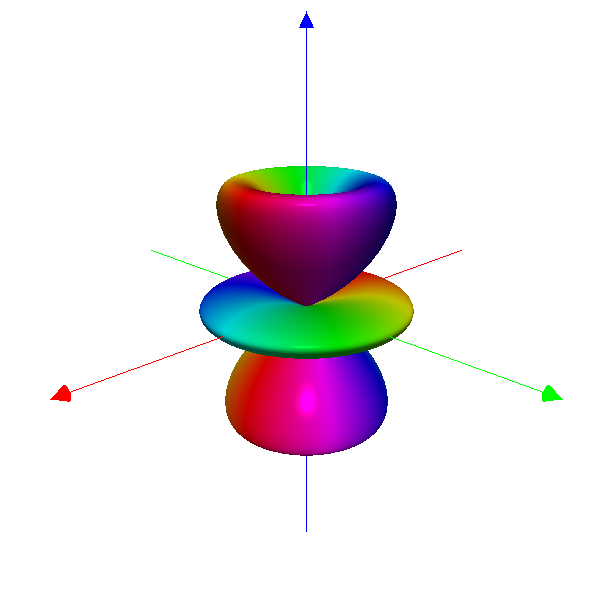
\includegraphics[width=0.14\textwidth,trim={0 3cm 0 -2cm},clip]{3m1} & 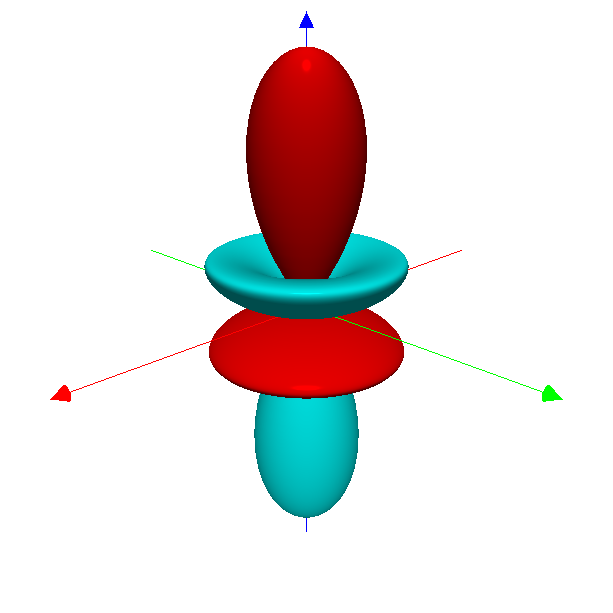
\includegraphics[width=0.14\textwidth,trim={0 3cm 0 -2cm},clip]{30} & 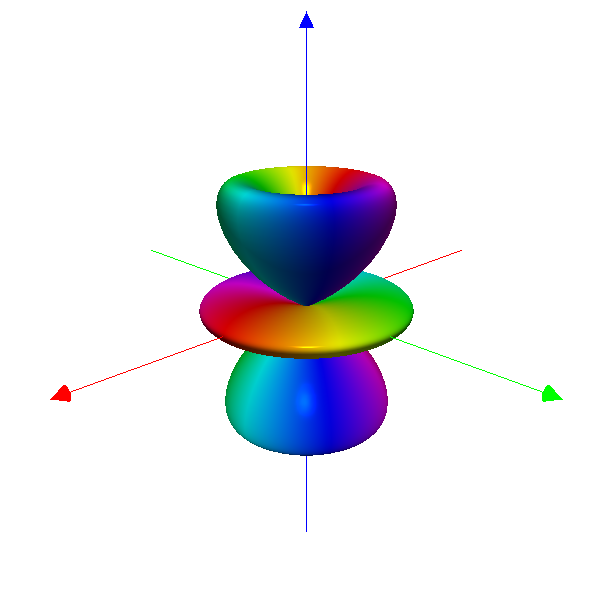
\includegraphics[width=0.14\textwidth,trim={0 3cm 0 -2cm},clip]{3p1} & 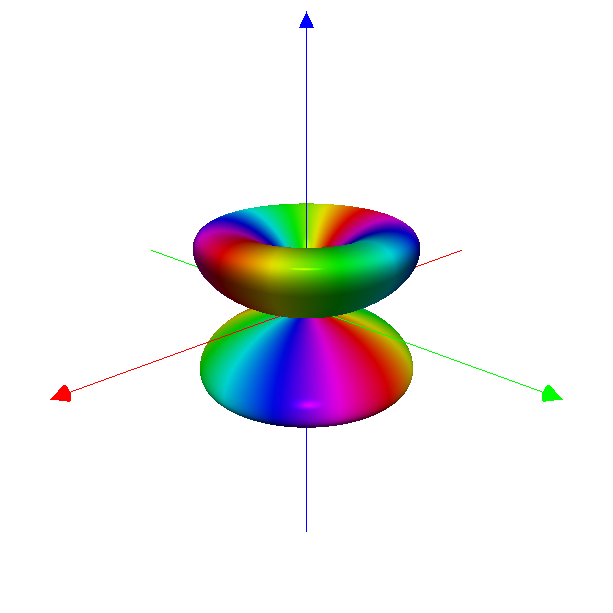
\includegraphics[width=0.14\textwidth,trim={0 3cm 0 -2cm},clip]{3p2} & 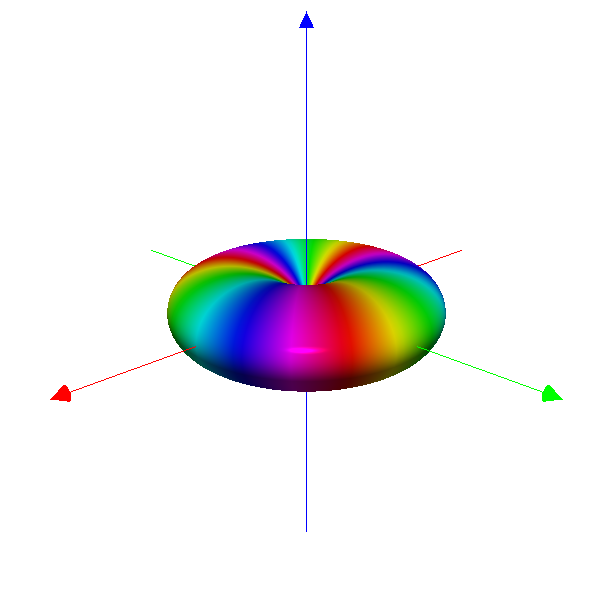
\includegraphics[width=0.14\textwidth,trim={0 3cm 0 -2cm},clip]{3p3} \\ 
$l=3,\;m=-3$ & $l=3,\;m=-2$ & $l=3,\;m=-1$ & $l=3,\;m=0$ & $l=3,\;m=1$ & $l=3,\;m=2$ & $l=3,\;m=3$
\end{tabular}
}
\end{minipage}
}
\end{center}
\end{table}
\clearpage
\begin{table}
\begin{center}
\small
\rotatebox{-90}{
\begin{minipage}{\textheight}
\caption{The first few real spherical harmonics.}
\label{table:realYlm}
\makebox[1.1\textheight]{
\begin{tabular}{c c c c c c c}
& & & 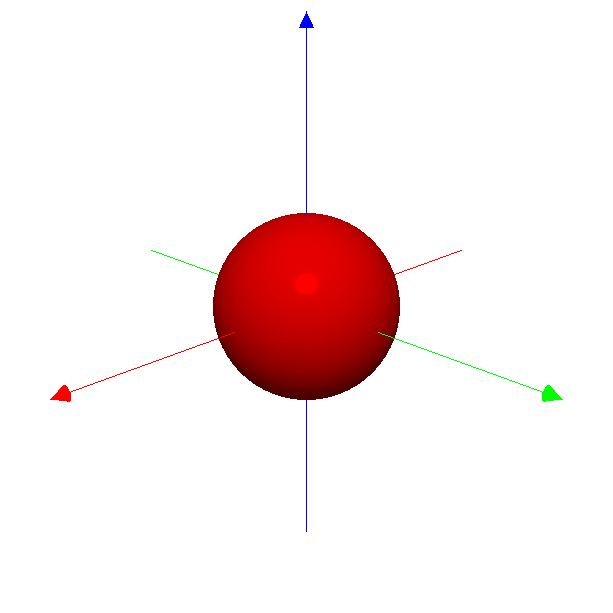
\includegraphics[width=0.14\textwidth,trim={0 3cm 0 -2cm},clip]{s} & & & \\
& & & $s$ & & & \\
& & 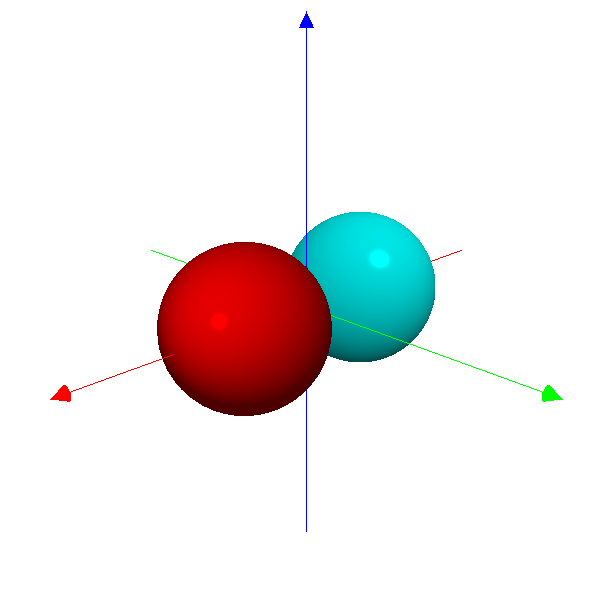
\includegraphics[width=0.14\textwidth,trim={0 3cm 0 -2cm},clip]{px} & 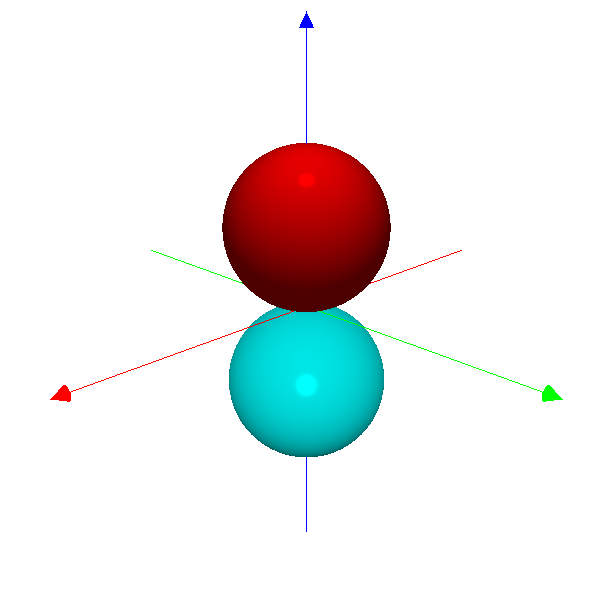
\includegraphics[width=0.14\textwidth,trim={0 3cm 0 -2cm},clip]{pz} & 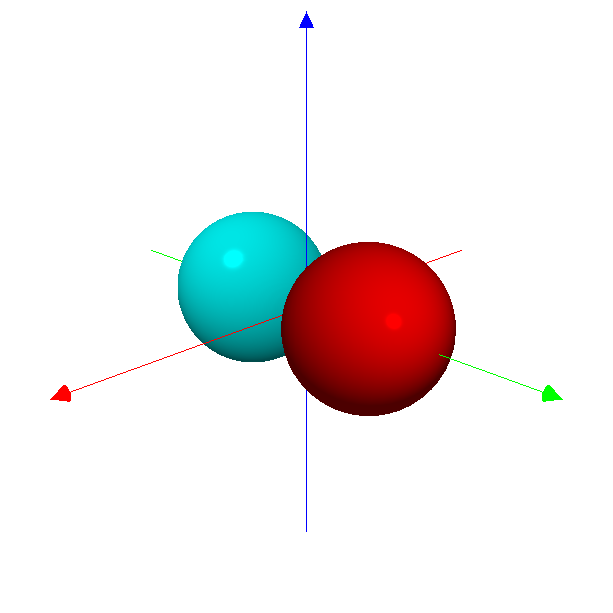
\includegraphics[width=0.14\textwidth,trim={0 3cm 0 -2cm},clip]{py} & & \\
& & $p_x$ & $p_z$ & $p_y$ & & \\
& 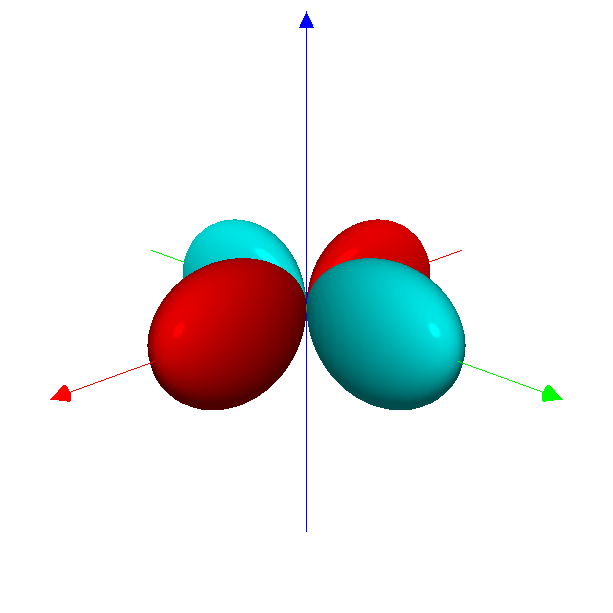
\includegraphics[width=0.14\textwidth,trim={0 3cm 0 -2cm},clip]{dxxyy} & 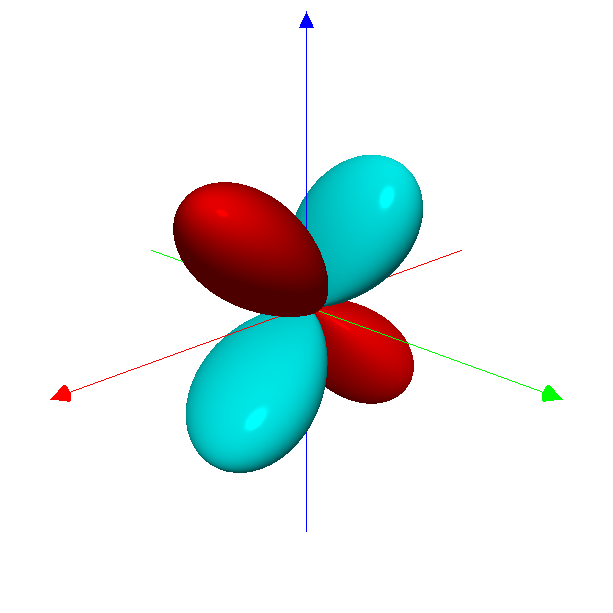
\includegraphics[width=0.14\textwidth,trim={0 3cm 0 -2cm},clip]{dxz} & 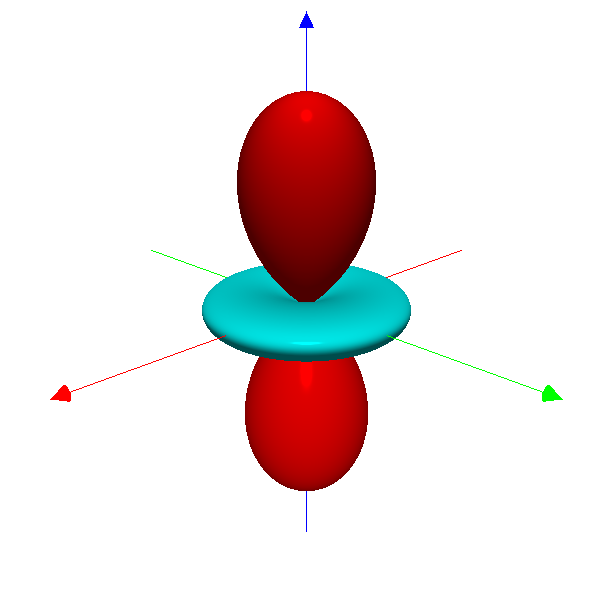
\includegraphics[width=0.14\textwidth,trim={0 3cm 0 -2cm},clip]{d3zz1} & 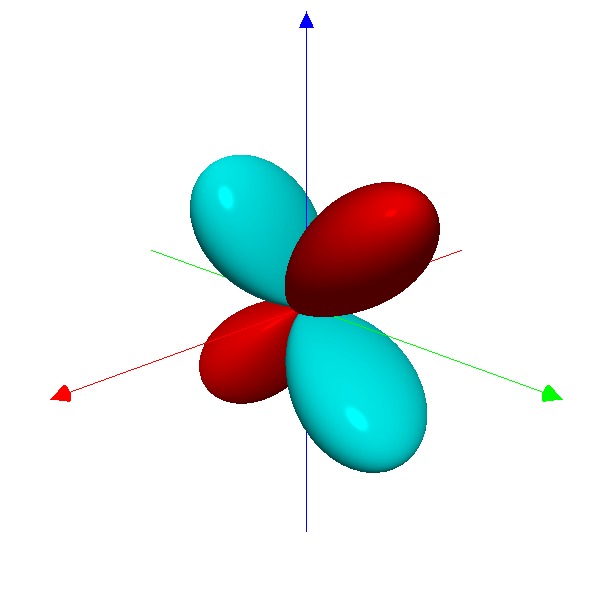
\includegraphics[width=0.14\textwidth,trim={0 3cm 0 -2cm},clip]{dyz} & 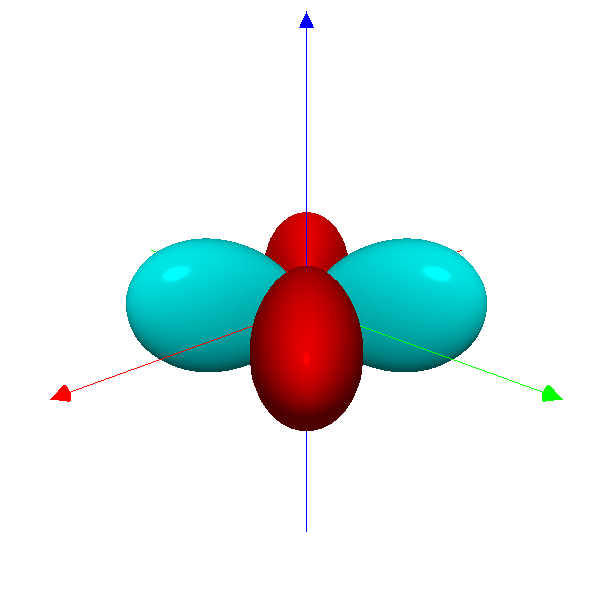
\includegraphics[width=0.14\textwidth,trim={0 3cm 0 -2cm},clip]{dxy} & \\
& $d_{x^2-y^2}$ & $d_{xz}$ & $d_{3z^2-1}$ & $d_{yz}$ & $d_{xy}$ & \\
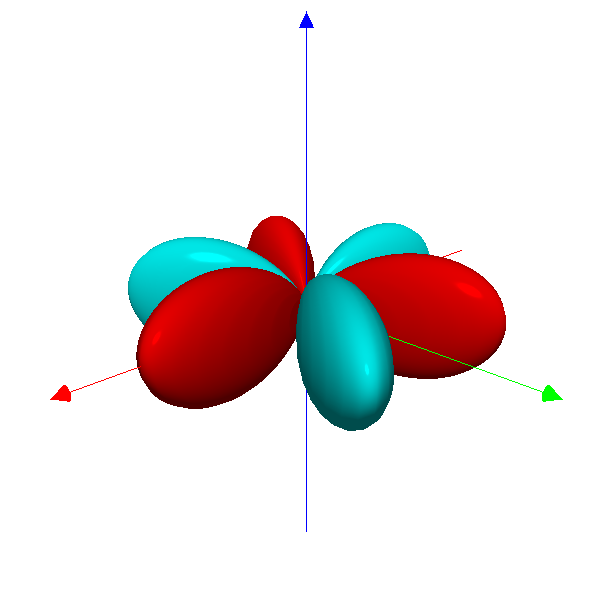
\includegraphics[width=0.14\textwidth,trim={0 3cm 0 -2cm},clip]{fxxx3yy} & 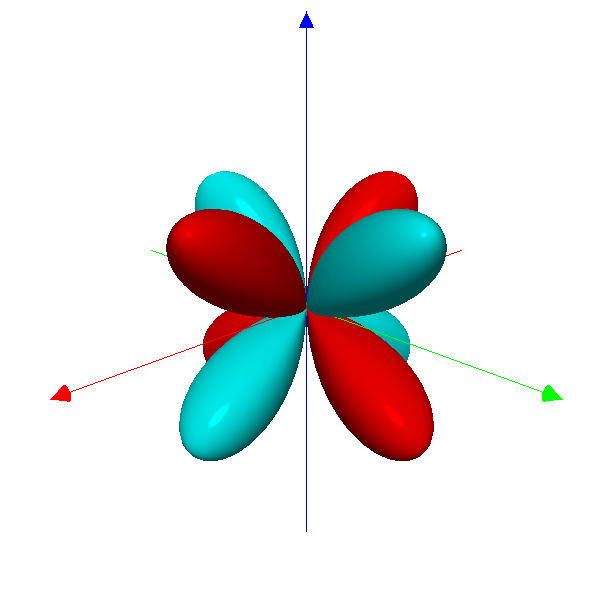
\includegraphics[width=0.14\textwidth,trim={0 3cm 0 -2cm},clip]{fzxxyy} & 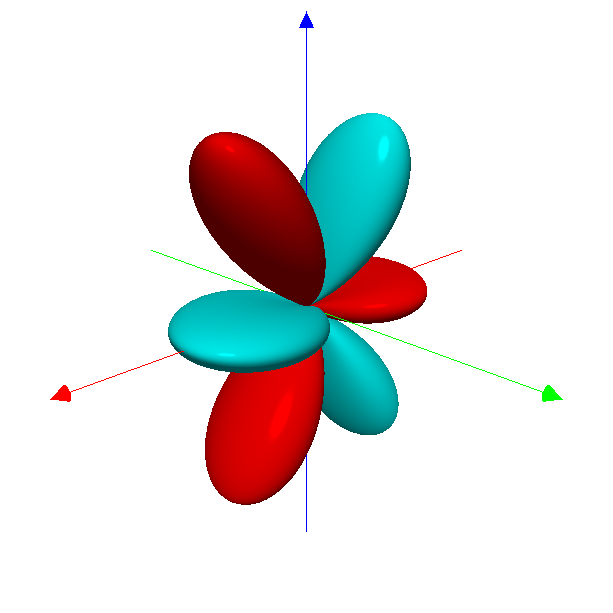
\includegraphics[width=0.14\textwidth,trim={0 3cm 0 -2cm},clip]{fx5zz1} & 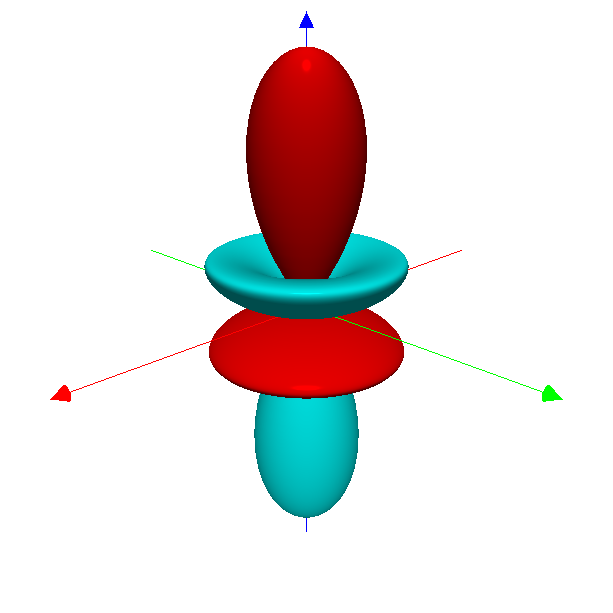
\includegraphics[width=0.14\textwidth,trim={0 3cm 0 -2cm},clip]{fz5zz3} & 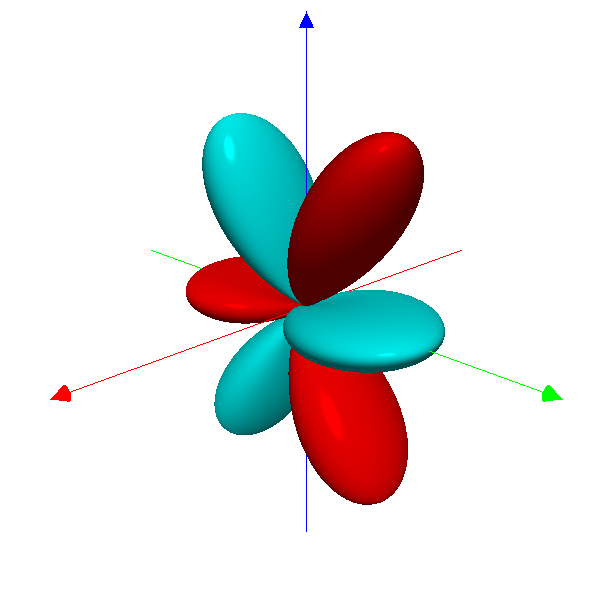
\includegraphics[width=0.14\textwidth,trim={0 3cm 0 -2cm},clip]{fy5zz1} & 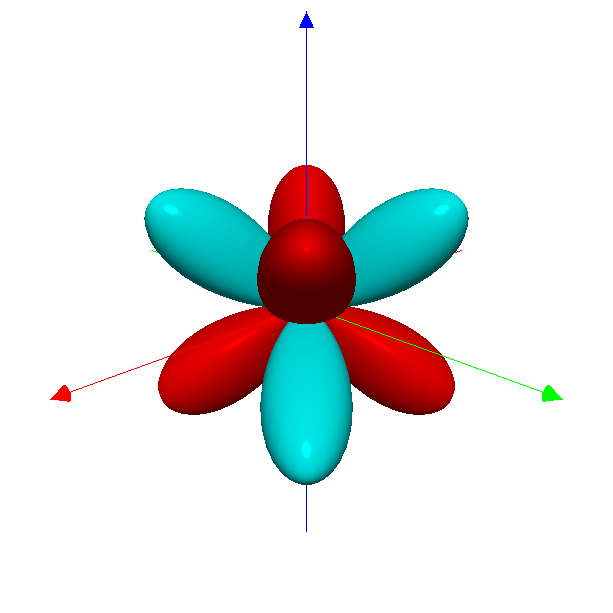
\includegraphics[width=0.14\textwidth,trim={0 3cm 0 -2cm},clip]{fxyz} & 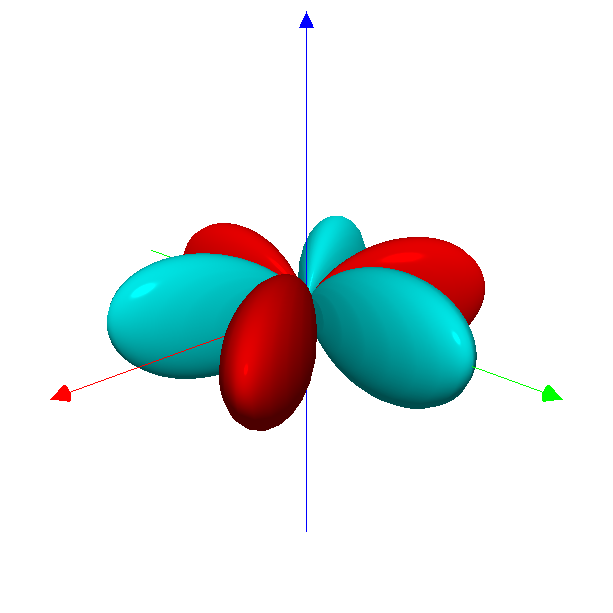
\includegraphics[width=0.14\textwidth,trim={0 3cm 0 -2cm},clip]{fy3xxyy} \\
$f_{x(x^2-3y^2)}$ & $f_{z(x^2-y^2)}$ & $f_{x(5z^2-1)}$ & $f_{z(5z^2-3)}$ & $f_{y(5z^2-1)}$ & $f_{xyz}$ & $f_{y(3x^2-y^2)}$ 
\end{tabular}
}
\end{minipage}
}
\end{center}
\end{table}
\clearpage

